%Template pembuatan proposal skripsi.
\documentclass{jtetiproposalskripsi}

%-----------------------------------------------------------------
%Disini awal masukan untuk data proposal skripsi
%---------- -------------------------------------------------------
\titleind{PENGEMBANGAN GATEWAY BERBASIS EMBEDDED DEVICE UNTUK INTEROPERABILITAS JARINGAN SENSOR NIRKABEL DAN PROTOKOL INTERNET}

\fullname{GUNTUR DHARMA}

\idnum{09/284593/TK/35393}

\approvaldate{13 November 2013}

\degree{Sarjana Teknik Elektro}

\yearsubmit{2013}

\program{Teknik Elektro}

\headprogram{Sarjiya, S.T., M.T., Ph.D.}

\dept{Teknik Elektro dan Teknologi Informasi}

\firstsupervisor{Sigit Basuki Wibowo, S.T., M.Eng.}
\firstnip{1976 0501 2002 12 1 002}

\secondsupervisor{Bimo Sunarfri Hantono, S.T., M.Eng.}
\secondnip{1977 0131 2002 12 1 003}


%-----------------------------------------------------------------
%Disini akhir masukan untuk data proposal skripsi
%-----------------------------------------------------------------

\begin{document}

\cover

\approvalpage

%-----------------------------------------------------------------
%Disini akhir masukan untuk muka skripsi
%-----------------------------------------------------------------

%-----------------------------------------------------------------
%Disini awal masukan Intisari
%-----------------------------------------------------------------
\begin{abstractind}
Penggunaan \emph{Wireless Sensor Network} (WSN) untuk gedung dan perumahan semakin populer karena dapat dimanfaatkan untuk berbagai kepentingan seperti \emph{home automation} dan \emph{home surveillance}. Oleh karena itu, untuk meningkatkan fleksibilitas penggunaan WSN, diperlukan sistem pengendalian yang dapat dikendalikan secara jarak jauh. Padahal pada umumnya, WSN dikendalikan oleh sebuah pengendali utama berada di sekitar tempat WSN itu berada.

Penelitian ini mengusulkan integrasi dari WSN dengan \emph{Internet Protocol} (IP) yang memungkinkan WSN dapat dikendalikan dimanapun dan dengan apapun asalkan masih terhubung dengan jaringan internet. Penelitian ini memanfaatkan infrastruktur jaringan data yang sangat populer dan terhubung ke internet, yaitu jaringan area lokal nirkabel atau dikenal dengan nama WiFi. Salah satu perangkat utama dalam jaringan WiFi adalah \emph{Access Point} (AP) yang berfungsi sebagai koordinator simpul. Selain itu, AP juga berfungsi sebagai gateway yang menghubungkan berbagai piranti yang terhubung padanya ke internet. Oleh karena itu, penelitian ini akan mengembangkan perangkat lunak yang akan ditanamkan ke dalam AP sehingga menjadikan AP mempunyai kemampuan sebagai gateway untuk kedua jaringan WiFi dan beberapa protokol WSN ke dalam jaringan internet.


\bigskip
\textbf{Kata kunci} : \emph{wireless sensor network}, \emph{internet protokol}, WiFi, interoperabilitas.
\end{abstractind}
%-----------------------------------------------------------------
%Disini akhir masukan Intisari
%-----------------------------------------------------------------

\tableofcontents
\addcontentsline{toc}{chapter}{DAFTAR ISI}
\selectlanguage{bahasa}\clearpage\pagenumbering{arabic}\setcounter{page}{1}

%-----------------------------------------------------------------
%Disini awal masukan untuk Bab
%-----------------------------------------------------------------
\chapter{LATAR BELAKANG}

\section{Latar Belakang Masalah}
Jaringan sensor nirkabel (\emph{Wireless Sensor Network}, WSN) adalah jaringan simpul (\emph{node}) sensor otonom terdistribusi yang digunakan untuk memonitor kondisi fisik atau lingkungan misalnya suhu, suara, getaran, kelembaban, dan lain-lain. Selain itu, tidak menutup kemungkinan untuk menambahkan fungsi tambahan pada setiap simpul misalnya port masukan/keluaran yang dapat digunakan sebagai pengendali aktuator yang terhubung ke piranti elektrik atau elektronis.

Penggunaan WSN untuk sebuah gedung dan rumah semakin populer karena dapat dimanfaatkan untuk berbagai kepentingan. Contoh penerapan WSN dalam rumah yang sangat populer adalah \emph{home surveillance} yaitu pemanfaatan WSN untuk mengawasi tiap sudut rumah secara \emph{realtime}. Dengan ini, sang pemilik rumah tidak perlu lagi khawatir karena rumahnya kurang pengawasan karena mengawasi rumah menjadi semakin mudah dengan bantuan WSN ini. Contoh lainnya adalah \emph{home automation} yaitu proses automatisasi segala urusan yang ada di rumah. Sebagai contoh, sang pemilik rumah harus menyalakan lampu di kala waktu sudah senja dan atau menyalakan pendingin ruangan saat pemilik baru saja pulang dari bekerja. Segala sesuatu yang mungkin untuk diautomatisasi, dapat terealisasi dengan bantuan WSN.

Pada umumnya, WSN dikendalikan oleh \emph{sink node} yang berada dekat pada wilayah jaringan sensornya. Sehingga permasalahan pada WSN adalah jika diinginkan pusat kendali berada pada tempat yang jauh dari jaringan sensornya. Solusi yang mungkin dari permasalahan ini adalah penggunaan \emph{Internet Protocol} (IP) karena jaringan IP sangat luas dan dapat diakses dimanapun dan dengan apapun.

Namun demikian, pada umumnya jaringan WSN tidak menggunakan IP, melainkan protokolnya sendiri, seperti protokol \emph{zigbee}. Oleh karena itu, diperlukan sebuah gateway yang mampu menghubungkan WSN dari berbagai macam \emph{vendor} dengan jaringan internet.



\section{Tujuan Penelitian}
Tujuan penelitian ini adalah mempelajari kemungkinan pengembangan perangkat lunak yang akan ditanamkan ke dalam sebuah \emph{access point} untuk difungsikan sebagai gateway sehingga mampu digunakan untuk mengintegrasikan jaringan WiFi dan beberapa protokol WSN ke jaringan internet.



\section{Manfaat Penelitian}
Dengan terhubungnya WSN ke jaringan internet dimungkinkan pengembangan aplikasi WSN yang dapat diakses melalui jaringan internet. Terhubungnya WSN ke jaringan internet akan membuka kemungkinan pengembangan layanan-layanan yang lebih beragam terutama layanan yang berbasis IP. Hal ini sejalan dengan perkembangan teknologi komunikasi yang menuju konvergensi penggunaan IP.

Selain itu, pengintegrasian gateway untuk WiFi dan WSN dalam satu piranti juga membuka peluang besar untuk memecahkan persoalan interoperabilitas perangkat keras dan kemudahan sistem.

%-------------------------------------------------------------------------------
\chapter{TINJAUAN PUSTAKA DAN DASAR TEORI}                

\section{Tinjauan Pustaka}
Secara umum, cara untuk menghubungkan WSN dengan jaringan internet dapat dikelompokkan menjadi dua. Cara pertama adalah menggunakan gateway dan cara yang kedua adalah dengan menggunakan simpul sensor yang sudah dilengkapi dengan protokol internet. Cara yang lebih mudah ditempuh adalah dengan cara yang pertama karena pengubahan yang dilakukan relatif tidak terlalu besar. Sedangkan cara yang kedua akan menemui banyak kendala terutama pada WSN yang sudah terpasang karena harus dilakukan penggantian tiap simpul sensor.

Salah satu usaha untuk mengintegrasikan jaringan WSN dengan jaringan WiFi menggunakan gateway misalnya dilakukan pada penelitian. Pada riset tersebut pengintegrasian dilakukan dengan sebuah komputer yang didedikasikan untuk keperluan tertentu. Penggunaan komputer khusus ini adalah hardware-solution yang membutuhkan biaya dan kerumitan sistem.

Riset pada juga menawarkan pengintegrasian dengan jaringan IP. Namun demikian di dalam riset ini diperlukan perubahan yang signifikan jika konfigurasi jaringan sensor nirkabel sudah terpasang. Simpul sensor yang digunakan harus diganti dengan simpul sensor yang mendukung IP. Hal ini jelas akan memakan biaya yang cukup besar dan tidak praktis untuk dilakukan. Terlebih lagi jika jumlah sensor yang terpasang jumlahnya cukup banyak.

Riset pada sudah berhasil mengembangkan sebuah AP menjadi gateway yang dapat digunakan untuk menghubungkan sebuah protokol WSN dengan jaringan IP. Protokol WSN yang digunakan adalah protokol dari IQRF. Penelitian tersebut kemudian dilanjutkan dengan penelitian yang sudah diterapkan dalam sistem domotic.

\section{Landasan Teori}
\subsection{\emph{Wireless Sensor Network}}
Jaringan sensor nirkabel (Wireless Sensor Network, WSN) adalah jaringan simpul sensor otonom yang terdistribusi digunakan untuk memonitor kondisi fisik atau lingkungan misalnya suhu, suara, getaran, kelembaban, dan lain-lain. Selain itu, tidak menutup kemungkinan untuk menambahkan fungsi tambahan pada setiap simpul misalnya port masukan/keluaran (I/O port) yang terdapat dalam setiap simpul dihubungkan dengan aktuator sehingga dapat digunakan untuk mengendalikan piranti elektrik atau elektronis.

Secara umum, WSN dapat diilustrasikan seperti Gambar \ref{wsn}. Pada gambar tersebut terlihat adanya beberapa simpul yang diwakili dengan titik berukuran kecil dan satu buah simpul yang diwakili dengan titik berukuran lebih besar. Titik yang berukuran kecil mewakili simpul sensor sedangkan titik yang berukuran besar mewakili gateway yang berfungsi menghubungkan jaringan sensor nirkabel dengan pengendali utama yang dalam gambar tersebut diwakili oleh sebuah komputer. Contoh sebuah simpul dari IQRF ditunjukkan pada Gambar \ref{iqrf}.

\begin{figure}[ht!]
  \centering
    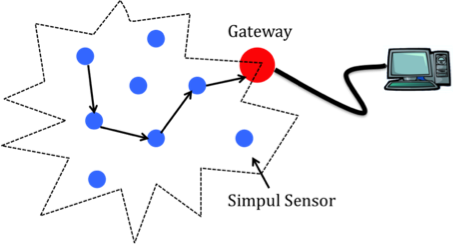
\includegraphics{gambar/wsn}
    \caption{Jaringan sensor nirkabel.}
    \label{wsn}
\end{figure}

Pada umumnya, WSN adalah jaringan yang berdiri sendiri. Untuk menghubungkan WSN dengan jaringan yang lain misalnya jaringan internet, maka salah satu cara adalah dengan membangun gateway WSN yang mampu menjembatani perbedaan protokol yang ada pada WSN dan jaringan internet. Cara tersebut adalah cara yang ditempuh dalam penelitian ini karena lebih mudah dilakukan dibandingkan dengan cara yang lain seperti sudah dijelaskan pada Bab Tinjauan Pustaka.

\begin{figure}[ht!]
  \centering
    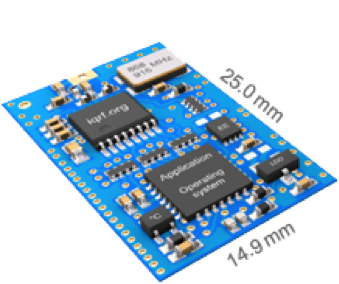
\includegraphics{gambar/iqrf}
    \caption{Contoh sebuah simpul sensor IQRF.}
    \label{iqrf}
\end{figure}

Sementara itu, jaringan WiFi sebagai jaringan lokal nirkabel yang digunakan untuk komunikasi data dalam suatu area lokal dan sudah tersebar di berbagai tempat. Lokal yang dimaksud disini adalah area yang tidak terlalu luas yaitu dengan radius sekitar 20m atau dalam sebuah gedung. Untuk membangun jaringan lokal menggunakan WiFi, perangkat utama yang digunakan adalah Access Point (AP). AP adalah piranti yang akan menjadi koordinator dalam jaringan lokal jika diinginkan topologi bintang (star) seperti diilustrasikan pada Gambar \ref{star}.

\begin{figure}[ht!]
  \centering
    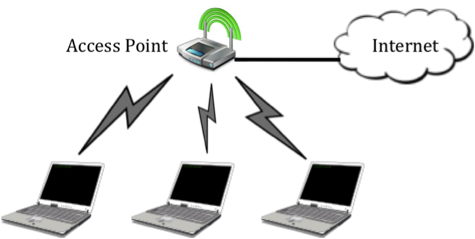
\includegraphics{gambar/star}
    \caption{Jaringan bintang menggunakan WiFi.}
    \label{star}
\end{figure}

Gambar \ref{star} memberi ilustrasi sebuah jaringan WiFi yang terdiri dari tiga buah komputer dan satu buah AP yang terhubung ke jaringan internet. Dengan konfigurasi tersebut, semua komputer yang ada di dalam jaringan WiFi dapat berkomunikasi dengan internet dengan aturan yang ditentukan oleh AP.

Jika dilihat lebih dalam lagi, AP ini sebenarnya adalah piranti tertanam (embedded device) yang didalamnya sudah terdapat pusat pengolahan utama, memory, dan penyimpanan (storage). Dengan kenyataan inilah maka AP mempunyai potensi untuk menjagi gateway bagi jaringan WiFi dan WSN ke jaringan internet. Untuk mengembangkan aplikasi yang akan ditanamkan ke dalam AP, maka diperlukan sistem operasi yang sesuai untuk AP.

\subsection{TCP/IP}
Protokol internet adalah kumpulan protokol-protokol komunikasi yang digunakan dalam internet dan jaringan komputer sejenis, dan umumnya merupakan protokol yang paling populer untuk WAN. Pada umumnya hal ini dikenal dengan TCP/IP, karena protokol utamanya merupakan protokol jaringan pertama yang terstandarisasi. Terkadang hal ini dikenal dengan model DoD karena pengaruh ARPANET pada dekade 1970an.

TCP/IP menyediakan konektivitas antar ujung yang menspesifikasikan bagaimana data harus diformat, dialamatkan, ditransmisikan, dirutekan, dan diterima di tujuan. TCP/IP memiliki empat layer abstraksi yang digunakan untuk mengurutkan semua protokol internet menurut jangkauan jaringan yang terlibat. Dari terendah sampai tertinggi, lapisan-lapisan tersebut adalah layer link, layer internet, layer transport, dan layer aplikasi.


\subsection{Web Server}
Web server dapat mengacu pada perangkat keras atau perangkat lunak yang membantu dalam penyampaian konten web yang dapat diakses melalui internet.

Penggunaan web server yang paling umum adalah sebagai host untuk halaman web, walaupun ada beberapa penggunaan lain seperti game, media penyimpan data, atau penjalanan aplikasi perusahaan.


\subsection{AJAX}
AJAX adalah kelompok dari teknik-teknik pengembangan web yang digunakan pada klien untuk membuat aplikasi asinkron. Dengan AJAX, aplikasi web dapat mengirim dan menerima data dari sebuah server secara asinkron tanpa mengganggu tampilan dari halaman yang ada. Data dapat diambil menggunakan obyek XMLHttpRequest. Penggunaan XML tidak diperlukan, malahan JSON lebih sering digunakan, dan rekues tidak harus asinkron.

AJAX bukanlah sebuah teknologi, tapi kelompok dari teknologi-teknologi. HTML dan CSS dapat digunakan dalam kombinasi untuk mark up dan informasi tampilan. DOM diakses oleh JavaScript untuk menampilkan dan mengijinkan pengguna untuk berinteraksi dengan informasi tertampil. JavaScript dan obyek XMLHttpRequest menyediakan sebuah metode untuk pertukaran data secara asinkron antara browser dan server untuk menghindari muat ulang halaman secara keseluruhan.


\subsection{OpenWRT}
OpenWRT adalah sebuah sistem operasi untuk \emph{embedded device} yang berbasis pada Linux kernel. OpenWRT pada umumnya digunakan dalam routing \emph{network traffic}. Komponen-komponen utamanya adalah Linux kernel, util-linux, uClibc dan BusyBox. Semua komponen sudah dioptimalkan dan dimampatkan untuk bisa muat dalam \emph{router} rumahan yang memiliki keterbatasan media penyimpan dan memori. OpenWRT dapat dikonfigurasikan melalui antarmuka \emph{command-line} (\emph{ash shell}), seperti dapat dilihat pada Gambar \ref{openwrt}, atau dengan antarmuka Web (LuCI). Terdapat kurang lebih 3.500 paket-paket perangkat lunak tambahan yang tersedia untuk diinstal melalui sistem manajemen paket \emph{opkg}.

\begin{figure}[ht!]
  \centering
    
\includegraphics[width=10cm]{gambar/openwrt}
    \caption{Tampilan antarmuka \emph{command-line} OpenWRT versi \emph{BackFire}.}
    \label{openwrt}
\end{figure}

OpenWRT dapat berjalan pada router CPE (\emph{Customer Premised Equipment}), \emph{gateway} residensial, komputer saku (seperti Ben NanoNote), dan komputer jinjing. OpenWRT juga dapat berjalan pada komputer konvensional atau komputer dengan arsitektur x86. Banyak \emph{patch} dari kode sesumber berbasis OpenWRT yang diubah kedalam Linux kernel utama.

%-------------------------------------------------------------------------------
\chapter{METODOLOGI}

\section{Alat dan Bahan}
Bahan yang digunakan dalam penelitian ini adalah:

\vspace{-0.5cm}

\begin{enumerate}[a.]
\begin{singlespace}
\itemsep0em
\item Kit pancar-rima (10 unit),
\item Kit pengembangan program (2 unit),
\item Kit pengunduh program (2 unit),
\item Asesoris kit pancar-rima (10 unit),
\item Kit ekspansi (5 unit),
\item Access Point (3 unit).
\end{singlespace}
\end{enumerate}

\section{Langkah Kerja}
Rancangan arsitektur yang akan digunakan pada penelitian ini diilustrasikan seperti pada Gambar \ref{wifi}. Pada gambar tersebut diilustrasikan sebuah sistem yang terdiri atas dua buah WSN dengan protokol yang berbeda dan satu buah jaringan nirkabel lokal (WiFi). Protokol WSN yang akan digunakan dalam penelitian ini adalah dari IQRF dan ZigBee. Pelaksanaan penelitian ini akan dibagi menjadi tiga paket pekerjaan (Work Package, WP).

\textbf{WP 1: Perancangan Perangkat Lunak}

Pada tahap ini akan dilakukan studi literatur yang dititikberatkan pada sistem operasi (Operating System, OS) untuk piranti tertanam (embedded device). Langkah selanjutnya adalah rerancangan perangkat lunak yang akan ditanamkan pada Access Point (AP). Perangkat lunak yang akan ditanamkan harus bekerja secara efisien karena kemampuan komputasi yang terbatas pada AP.

\begin{figure}[ht!]
  \centering
    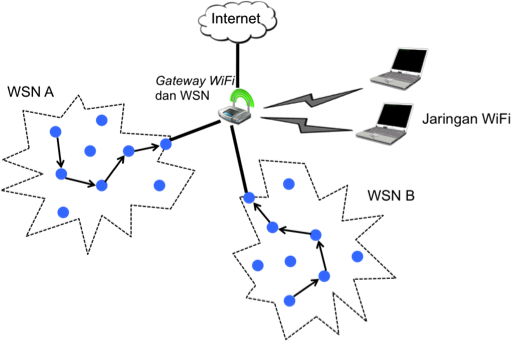
\includegraphics{gambar/wifi}
    \caption{Arsitektur WSN dan WiFi dengan sebuah AP.}
    \label{wifi}
\end{figure}

\textbf{WP 2: Implementasi Perangkat Lunak}

Implementasi perangkat lunak dilakukan pada tahap ini. Langkah pertama yang dilakukan adalah memastikan bahwa WSN dapat terhubungan dengan internet sesuai dengan yang direncanakan. Langkah selanjutnya adalah memastikan bahwa jaringan WiFi tidak mengalami gangguan setelah perangkat lunak yang baru tertanam pada AP. Penambahan layanan-layanan yang diperlukan dapat pula dilakukan pada tahap ini.

\textbf{WP 3: Integrasi dan Pengujian Seluruh Sistem}

Jika jaringan WiFi dan dua protokol WSN masing-masing dapat berhubungan dengan internet, maka pada tahap ini akan dilakukan pengujian sistem secara keseluruhan. Pengujian dinaikkan dari skala lab menjadi skala \emph{test-bed}. Pengujian dalam \emph{test-bed} dilakukan untuk menjamin bahwa sistem yang dikembangkan bekerja sesuai dengan yang direncanakan.

\section{Jadwal Kegiatan}
Penelitian direncanakan akan dilaksanakan selama enam bulan. Rincian rencana jadwal penelitian dicantumkan dalam tabel berikut.

\begin{center}
Tabel 3.1. Jadwal Penelitian.
\end{center}
\vspace{-0.5cm}
\begin{figure}[ht!]
  \centering
    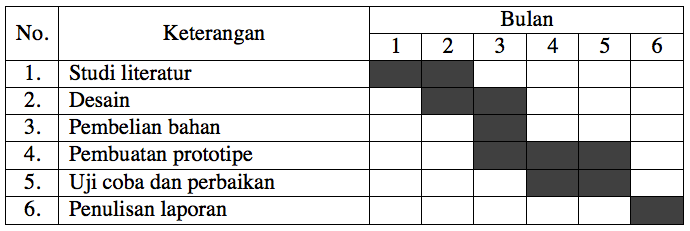
\includegraphics[width=13cm]{gambar/timeline}
\end{figure}

%-----------------------------------------------------------------
%Disini akhir masukan Bab
%-----------------------------------------------------------------

%-----------------------------------------------------------------
%Disini awal masukan untuk Daftar Pustaka
%-----------------------------------------------------------------
%%\nocite{Abel2010,Guerbas201350}
%%\bibliography{research-plan}
%%\bibliographystyle{plainnat}
\begin{thebibliography}{9}

\bibitem[satu(2013)]{satu01}
Spinar, R., dkk, ``Demo Abstract: Efficient Building Management with IP- based Wireless Sensor Network'', , 6th European Conference on Wireless Sensor Networks. Cork, Ireland 11-13 February 2009.

\bibitem[dua(2013)]{dua02}
Adam Dunkels, Thiemo Voigt, Niclas Bergman, dan Mats Jonsson ``The Design and Implementation of an IP-based Sensor Network for Intrusion Monitoring'', Swedish National Computer Networking Workshop, Sweden, 2004.

\bibitem[tiga(2013)]{tiga03}
Sigit B. Wibowo, dan Widyawan, ``Wireless Sensor Network and Internet Protocol Integration with COTS'', 2013 AUN/SEED-Net Regional Conference in Electrical and Electronics Engineering, Bangkok, Thailand, 2013.

\bibitem[empat(2013)]{empat04}
Dokumen online, http://www.iqrf.org/, IQRF, diakses pada Maret 2013

\bibitem[lima(2013)]{lima05}
Widyawan, Sigit B. Wibowo, dkk, ``iHome: Low-Cost Domotic for Residential Houses'', 5th AUN/SEED-Net Regional Conference on Information and Communications Technology (RCICT), Manila, Filipina, 2012.

\bibitem[enam(2013)]{enam06}
Dokumen online,https://openwrt.org/, diakses pada Maret 2013

\bibitem[tujuh(2013)]{tujuh07}
Dokumen online, http://www.digi.com/technology/rf-articles/wireless-zigbe,
diakses pada Maret 2013.

\end{thebibliography}
\addcontentsline{toc}{chapter}{DAFTAR PUSTAKA}
%-----------------------------------------------------------------
%Disini akhir masukan Daftar Pustaka
%-----------------------------------------------------------------

\end{document}